\subsection{Coordinate Transformations \hfill(Release 1/2017)}

Cartesian coordinates are not the only coordinate system that MSE graduate students will encounter in the core. Cylindrical coordinates and spherical coordinates are both useful in, for example, describing stress and strain fields around dislocations and vacancies.

\paragraph{Cartesian} coordinates, as mentioned in Sec. \ref{subsec:Tensors} utilize an orthogonal basis set and are often the easiest to use when describing and visualizing vector operations and physical laws. The rank-2 stress tensor (introduced in Sec. \ref{subsec:Tensors}) is represented using the following $3 \times 3 \times 3$ matrix and is shown in Fig.~ \ref{fig:StressTensors}:

\begin{figure}%
	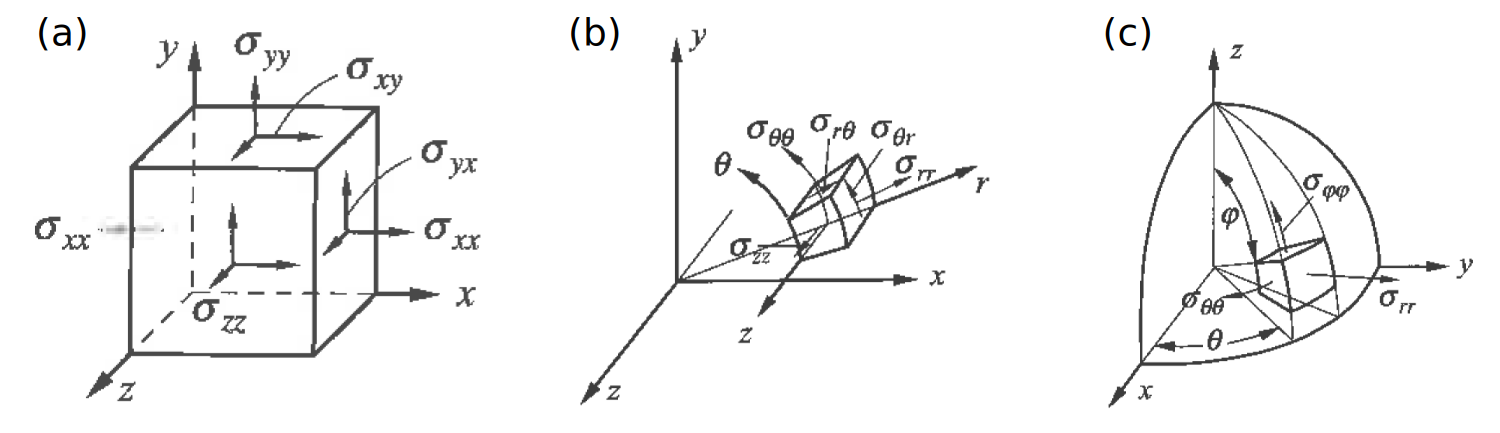
\includegraphics[scale=0.4]{StressTensors}%
	\caption{Stress tensors for (a.) Cartesian, (b.) cylindrical, and (c.) spherical coordinate systems. From Nix and Cai.}%
	\label{fig:StressTensors}%
\end{figure}

\begin{equation}
	\sigma_{ij}
	\begin{bmatrix}
		\sigma_{xx} & \sigma_{xy} & \sigma_{xz}\\
    \sigma_{yx} & \sigma_{yy} & \sigma_{yz}\\
    \sigma_{zx} & \sigma_{zy} & \sigma_{zz}\\
	\end{bmatrix}
	\label{eq:CartesianStressTensor}
\end{equation}

\paragraph{Cylindrical} coordinates are also an orthogonal coordinate system defined in Fig. \ref{fig:StressTensors}(b). The stress tensor in this coordinate system is defined by the cylinderical components $r$, $\theta$, and $z$. Here, $r$ is the distance from the $z$-axis to the point. $\theta$ is the angle between the reference direction (we use the $x$-direction) and the vector that points from the origin to the coordinates projected onto the $xy$ plane. $z$ is the distance from the point's coordinates projected onto $xy$ plane and the point itself. The stress tensor is represented as  

\begin{equation}
	\sigma_{ij}=
	\begin{bmatrix}
		\sigma_{rr} & \sigma_{r \theta} & \sigma_{r z}\\
    \sigma_{\theta r} & \sigma_{\theta\theta} & \sigma_{\theta z}\\
    \sigma_{z r} & \sigma_{z \theta} & \sigma_{zz}\\
	\end{bmatrix}
	\label{eq:CylindricalStressTensor}
\end{equation}

\paragraph{Spherical} coordinates are defined by $r$, $\theta$ and $\phi$. Here $r$ is the radial distance from the origin to the point. $\theta$ is the polar angle, or the angle between the $x$-axis and the point, projected onto the $xy$ plane. $\phi$ is the azimuthal angle, or the angle between the $z$-axis and the vector pointing from the origin to the point. The stress tensor is

\begin{equation}
	\sigma_{ij}=
	\begin{bmatrix}
		\sigma_{rr} & \sigma_{r \theta} & \sigma_{r \phi}\\
    \sigma_{\theta r} & \sigma_{\theta\theta} & \sigma_{\theta \phi}\\
    \sigma_{\phi r} & \sigma_{\phi \theta} & \sigma_{\phi\phi}\\
	\end{bmatrix}
	\label{eq:SphericalStressTensor}
\end{equation}

We will often want to transform tensor values from one coordinate system to another in ${\rm I\!R}^3$. As an example, we will convert the stress state from a cylinderical coordinate system to a Cartesian coordinate system. This transformation from stress state in the original coordinate system ($\sigma_{kl
} = \sigma_{kl}^{r \theta z}$) to the new coordinate system ($\sigma_{ij
}^{'} = \sigma_{ij}^{xyz}$) is performed using the following relationship:

\begin{equation}
	\sigma_{ij}' = Q_{ik}Q_{jk}\sigma_{kl}
	\label{eq:GeneralTransform}
\end{equation}

Where the summation notation (Sec. \ref{sec:SummationNotation}) is implicit. In our example the indices $kl$ indicate the original cylindrical coordinate system ($r$, $\theta$, $z$) and the indices $ij$ indicate the new coordinate system ($x$, $y$, $z$).

Note that Eq. \ref{eq:GeneralTransform} can be written in matrix form as:

\[\sigma = Q \cdot \sigma \cdot Q^{T}\]

The $Q$ matrix is defined the dot products between the unit vectors in the coordinate systems of interest. In simplified 2D transformation from polar to Cartesian, there is no $z$ component in either coordinate system and terms with those indices can be dropped.

%\begin{multline}
	%Q_{ik} \equiv (\hat{e}_{i}^{xyz} \cdot \hat{e}_k^{r \theta z}) =
	%\begin{bmatrix}
		%(\hat{e}_{x} \cdot \hat{e}_{r}) & (\hat{e}_{x} \cdot \hat{e}_{\theta}) & (\hat{e}_{x} \cdot \hat{e}_{z})\\
		%(\hat{e}_{y} \cdot \hat{e}_{r}) & (\hat{e}_{y} \cdot \hat{e}_{\theta}) & (\hat{e}_{y} \cdot \hat{e}_{z})\\
		%(\hat{e}_{z} \cdot \hat{e}_{r}) & (\hat{e}_{z} \cdot \hat{e}_{\theta}) & (\hat{e}_{z} \cdot \hat{e}_{z})\\
	%\end{bmatrix}\\
	%%Q_{jl} \equiv (\hat{e}_{j}^{xyz} \cdot \hat{e}_l^{r \theta z}) \\
%\end{multline}

\begin{equation}
	Q_{ik} \equiv (\hat{e}_{i}^{xy} \cdot \hat{e}_k^{r \theta}) =
	\begin{bmatrix}
		(\hat{e}_{x} \cdot \hat{e}_{r}) & (\hat{e}_{x} \cdot \hat{e}_{\theta})\\
		(\hat{e}_{y} \cdot \hat{e}_{r}) & (\hat{e}_{y} \cdot \hat{e}_{\theta})\\
	\end{bmatrix}\\
	%Q_{jl} \equiv (\hat{e}_{j}^{xyz} \cdot \hat{e}_l^{r \theta z}) \\
\end{equation}

where $\hat{e}_{r}$ and $\hat{e}_{\theta}$ is related geometrically to $\hat{e}_{x}$ and $\hat{e}_{y}$:

\begin{equation}
	\begin{bmatrix}
		\hat{e}_{r} = \hat{e}_{x} \cos(\theta) + \hat{e}_{y} \sin(\theta)\\
		\hat{e}_{\theta} = -\hat{e}_{x} \sin(\theta) + \hat{e}_{y} \cos(\theta)\\
	\end{bmatrix}\\
	%Q_{jl} \equiv (\hat{e}_{j}^{xyz} \cdot \hat{e}_l^{r \theta z}) \\
\end{equation} 

And therefore: 
\begin{align}
	Q_{ik} &\equiv (\hat{e}_{i}^{xy} \cdot \hat{e}_k^{r \theta}) =
	\begin{bmatrix}
		(\hat{e}_{x} \cdot \hat{e}_{r}) & (\hat{e}_{x} \cdot \hat{e}_{\theta})\\
		(\hat{e}_{y} \cdot \hat{e}_{r}) & (\hat{e}_{y} \cdot \hat{e}_{\theta})\\
	\end{bmatrix}
	=
	\begin{bmatrix}
		Q_{xr} & Q_{x\theta}\\
		Q_{yr} & Q_{y\theta}\\
	\end{bmatrix} \\
	&=
		\begin{bmatrix}
		\left(\hat{e}_{x} \cdot \left[\hat{e}_{x} \cos(\theta) + \hat{e}_{y} \sin(\theta)\right]\right) & \left(\hat{e}_{x} \cdot \left[-\hat{e}_{x} \sin(\theta) + \hat{e}_{y} \cos(\theta)\right]\right)\\
		\left(\hat{e}_{y} \cdot \left[\hat{e}_{x} \cos(\theta) + \hat{e}_{y} \sin(\theta)\right]\right) & \left(\hat{e}_{y} \cdot \left[-\hat{e}_{x} \sin(\theta) + \hat{e}_{y} \cos(\theta)\right]\right)	
		\end{bmatrix}\\
		&=
		\begin{bmatrix}
		\cos(\theta) & -\sin(\theta)\\
		\sin(\theta) & \cos(\theta)	
		\end{bmatrix}
\end{align}

So, to convert the stress tensor in polar coordinates ($\sigma_{kl}^{r\theta}$) to Cartesian ($\sigma_{ij}^{xy}$), we take the triple dot-product:

\begin{align}
	\sigma' &= Q \cdot \sigma \cdot Q^{T} =
	\begin{bmatrix}
		\sigma_{xx} & \sigma_{xy}\\
		\sigma_{yx} & \sigma_{yy}
	\end{bmatrix}=
	\begin{bmatrix}
		\cos(\theta) & -\sin(\theta)\\
		\sin(\theta) & con(\theta)	
	\end{bmatrix}\cdot
	\begin{bmatrix}
		\sigma_{rr} & \sigma_{r\theta}\\
		\sigma_{\theta r} & \sigma_{\theta \theta}
	\end{bmatrix}
\cdot
	\begin{bmatrix}
		\cos(\theta) & \sin(\theta)\\
		-\sin(\theta) & con(\theta)	
	\end{bmatrix}
	%&=
	%\begin{bmatrix}
	%\cos(\theta) (\sigma_{rr} \cos(\theta) - \sigma_{\theta r} \sin(\
%\theta)) - \sin(\theta)(\sigma_{r\theta}\cos(\theta) - \sigma_{\theta\theta}\sin(\theta) & \sin(\theta) (\sigma_{rr} \cos(\theta) - \sigma_{\theta r} \sin(\
%\theta)) + \cos(\theta)(\sigma_{r\theta}\cos(\theta) - \sigma_{\theta\theta}\sin(\theta)\\
	%\cos(\theta) (\sigma_{\theta r} \cos(\theta) + \sigma_{rr} \sin(\
%\theta)) - \sin(\theta)(\sigma_{\theta \theta}\cos(\theta) + \sigma_{r\theta}\sin(\theta) & \sin(\theta) (\sigma_{\theta r} \cos(\theta) + \sigma_{rr} \sin(\
%\theta)) + \cos(\theta)(\sigma_{\theta \theta}\cos(\theta) + \sigma_{r\theta}\sin(\theta)
	%\end{bmatrix}
\end{align}

Completing the math yields:
\begin{align}
	\sigma_{xx} &= \cos(\theta) \left[\sigma_{rr} \cos(\theta) - \sigma_{\theta r} \sin(
\theta)\right] - \sin(\theta)\left[\sigma_{r\theta}\cos(\theta) - \sigma_{\theta\theta}\sin(\theta)\right]\\
	\sigma_{xy} &= \sin(\theta) \left[\sigma_{rr} \cos(\theta) - \sigma_{\theta r} \sin(
\theta)\right] + \cos(\theta)\left[\sigma_{r\theta}\cos(\theta) - \sigma_{\theta\theta}\sin(\theta)\right]\\
	\sigma_{yx} &= \cos(\theta) \left[\sigma_{\theta r} \cos(\theta) + \sigma_{rr} \sin(
\theta)\right] - \sin(\theta)\left[\sigma_{\theta \theta}\cos(\theta) + \sigma_{r\theta}\sin(\theta)\right]\\
	\sigma_{yy} &= \sin(\theta) \left[\sigma_{\theta r} \cos(\theta) + \sigma_{rr} \sin(
\theta)\right] + \cos(\theta)\left[\sigma_{\theta \theta}\cos(\theta) + \sigma_{r\theta}\sin(\theta)\right]
\end{align}

In as system with only one or two stress components these coordinate transformations simplify greatly. Remember, though, in ${\rm I\!R}^3$ there will be $N = 3^2$ components due to increased dimentionality.
		
	%Q_{jl} \equiv (\hat{e}_{j}^{xyz} \cdot \hat{e}_l^{r \theta z}) \\

	%\subsubsection{Vector Calculus \hfill(Release TBD)}
	%
	%\textit{\textbf{Encountered in: MAT\texttt{\_}SCI 406, 408}} 